\label{chip}
\begin{titlepage}

\section{Pixel detectors}

\subsection{Brief overview}
\subsubsection{Signal formation}
When a charge particle passes through a pixel and loses energy by ionization a part of that energy is used to generate electron-hole pairs (some of the energy is also used for other processes, as the lattice excitation) which are then separated by the elettric field and collected at their respectivelly electrodes ($p$ for holes and $n$ for electrons)\footnote{Even if in principle both the electrode can be used to read a signal, for pixel detectors, where the number of channel and the complexity of readout are high, only one is actually used. In strip and pad detectors, instead, is more common a dual-side readout}; by the drift of these charges, a signal $i_e$ is generated on the  electrode $e$ as stated by the Ramo's theorem: 
\begin{equation}
   i_e(t) = -q v(t) E_{WF,e}
\end{equation}
where $v(t)$ is the instantaneous velocity of the charge $q$ and $E_{WF}$ is the weighting field, that is the field obtained biasing the electrode $e$ with 1V and all the others with 0V.\\
The drift velocity of the charge depends on the elettric field and on the mobility of the particle:
\begin{equation}
   v = \mu(E) E
\end{equation}
where $\mu(E)$ is a function of the electric field and is linear with $E$ only for small $E$: at highter values the probability
of interactions with optical phonons increases and the mobility drops and this leads to an indipendency of the velocity from the electric field (fig. \ref{fig:mobility_drift})\\
\begin{figure}[h!]
   \begin{subfigure}{.5\textwidth}
     \centering
     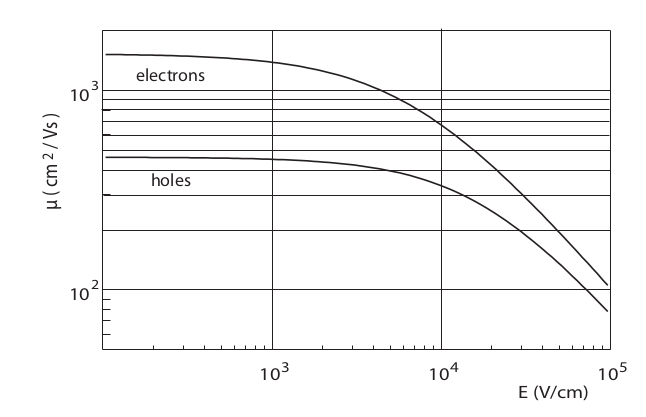
\includegraphics[width=.8\linewidth]{figures/mobility_in_semiconductor.png}
     \caption{Typical values for elecrons and holes mobility 
     in silicon at room temperature are $\mu _n \sim$ 1450 $cm^2/Vs$, $\mu _h = 500$}
     \label{fig:sfig1}
   \end{subfigure}%
   \begin{subfigure}{.5\textwidth}
     \centering
     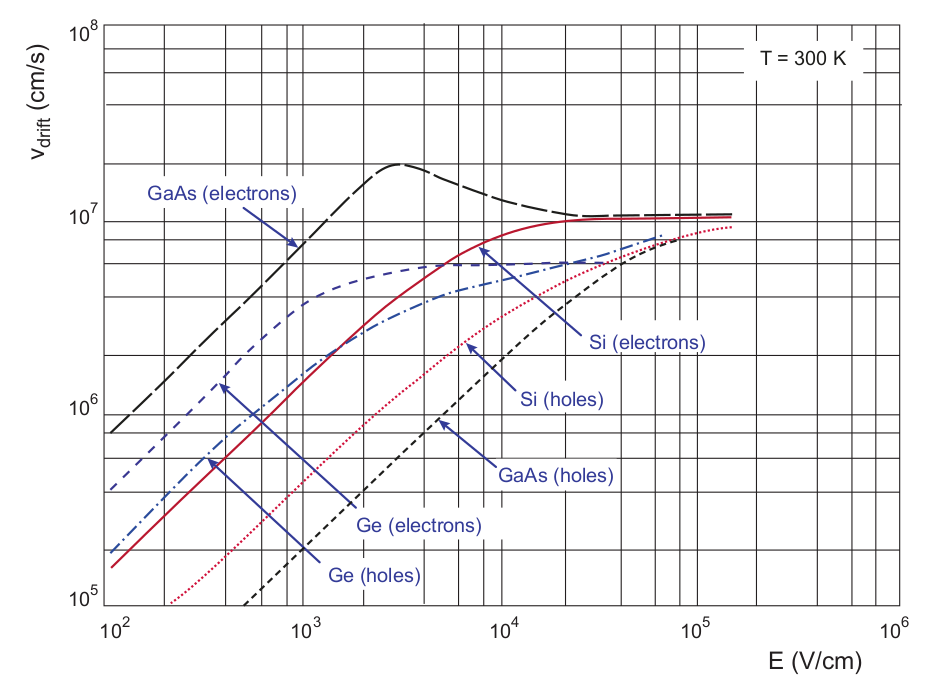
\includegraphics[width=.8\linewidth]{figures/velocity_in_semiconductor.png}
     \caption{Drift velocity at room temperature in different semiconductors}
     \label{fig:sfig2}
   \end{subfigure}
   \label{fig:mobility_drift}
\end{figure}

The average energy needed to create a pair at 300 K in silicon is $w_i$ = 3.65 eV, that is more than the mean ionization energy because of the interactions with phonon, hence for a MIP the most probable value of charge released is: 
\begin{equation}
   \langle \frac{dE}{dx}\rangle \frac{1}{w_i} = HOW \frac{fC}{\mu m} \sim electrons
\end{equation}
That is foundamental that pairs e/h are produced in the depleted region of the semiconductor where the probability of recombination with charge carriers is low.\\
Pixel detectors are then commonly reverse biased (a positive bias is given to the $n$ electrode and a negative to the $p$) and the depletion zone is grown in the epitaxial layer below the electrode; the depletion region is related with the extern bias $V_{ext}$, the resistivity $\rho$ and also with the dopant:
\begin{multicols}{2}
\begin{equation}
   d_{n} \sim 0.55 \sqrt{\frac{\rho}{\Omega cm}\frac{V_{ext}}{V}} \mu m 
\end{equation}\break
\begin{equation}
   d_{p} \sim 0.32 \sqrt{\frac{\rho}{\Omega cm}\frac{V_{ext}}{V}} \mu m
\end{equation}
\label{eq:deplation_d}
\end{multicols}
Looking at this formula one could think that high resistivity\footnote{Hight resistivity crystall can be produces using Czochralki (Cz) or float-zone (Fz) process; the fist one creates a silicon bulk with a highter oxygen concentration which can be beneficial for radiation damage} bulk are prefered, but instead for high radiation applications the starting resistivity is not too crucial and intermediate resisistivity (100 $\Omega$cm-1k$\Omega$cm) may be advantageous because the charges collection properties don't change so much during sensor lifetime while the effective space charge concentration changes after irradiation. IMMAGINE?\\

\subsubsection{Radiation dameges}
Radiation hardeness is a fundamental requirement for pixels detector especially in HEP since they are almost always installed near the interaction point where there is a high energy level of radiation.
Here the high fluence of particles can cause a damage both in the substrate of the detector and in the superficial electronics.\\
At LHC the $\phi_{eq}$\footnote{The radiation damage has a principal non ionising nature (non ionizing energy loss, NIEL) since the dislocation of the lattice is caused by the collision with nuclei; as stated by the NIEL hypothesis the subsrate damage is normalized to the damage caused by 1 MeV neutrons.} per year in the innermost pixels detector is $10^{14} n_{eq}/cm^2$; this number reduces by an order allontanandosi andando a prendere gli ultimi layer nel tracciatore. (referenza: pag 341 Wermes)\\
Dei secondi ..\\
Let's stop for a while on the substrate damages: the general result is the creation of new energy levels within the silicon band gap and depending on their energy-location their effect can be different (fig. \ref{fig:radiation_damage_scheme}). 
\begin{figure}
   \begin{subfigure}{.5\textwidth}
     \centering
     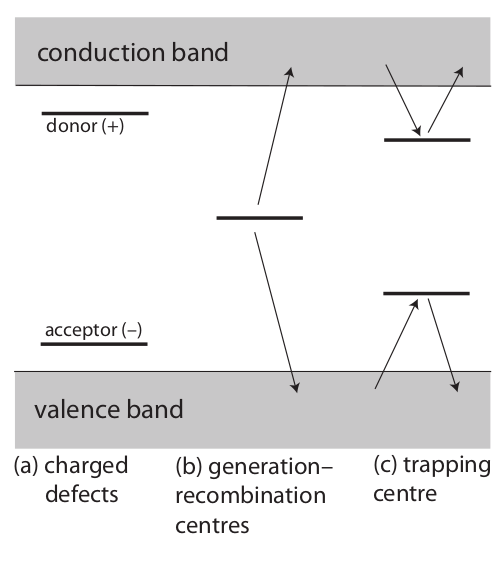
\includegraphics[width=.8\linewidth]{figures/radiation_damage_scheme.png}
     \caption{Three main type of defects produced by radiation}
     \label{fig:radiation_damage_scheme}
   \end{subfigure}%
   \begin{subfigure}{.5\textwidth}
     \centering
     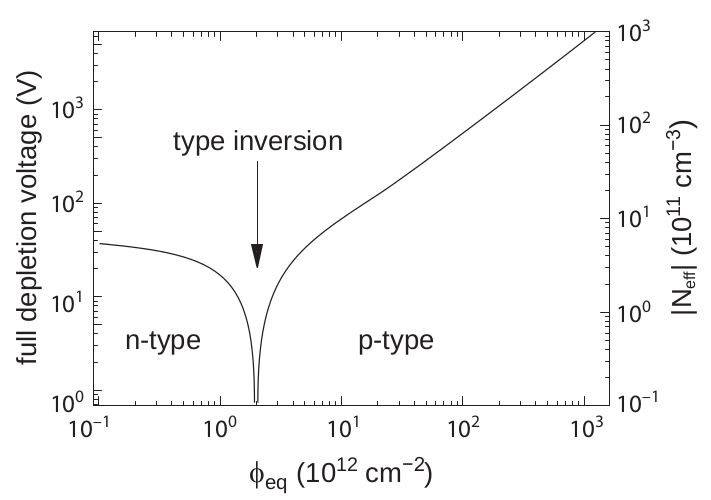
\includegraphics[width=.8\linewidth]{figures/type_inversion.png}
     \caption{1b}
     \label{fig:type_inversion}
   \end{subfigure}
\end{figure}
The three main consequence, corresponding with the tre main substrate defects and corresponding with processes described in the Shockely-Read-Hall (SRH) statistics, of radiation damage are the changing of the effect doping concentration, the leakage current and the increasing of trapping probability.\\
\textbf{Changing of the effective doping concentration:} is associated with the creation/removal of donors and acceptors center which trap respectively electrons/holes from the conduction band and cause a change in effective space charge density. Even an inversion (p-type becomes n-type) can happen: indeed it is quite common at not too high fluences ($\phi_{eq} 10^{12-13}n_{eq}cm^{-2}$). \\
A changing in the doping concentration requires an adjust of the biasing of the sensor in time (eq.\ref{eq:deplation_d}) and sometimes can be difficult keeping to fully deplete the bulk.\\
Studies have shown that, compared to p+ -in-n sensors (easier and chieper to obtain), n+ -in-p sensors are more radiation hard ando also, since they are already p-type, they don't invert.\\
\textbf{Leakage current:} is associated with the generation-recombination centres. It has a strong dependence with the temperature ($I_{leak}\propto T^2$), whose solution is therefore to operate at lower temperature.\\
\textbf{Increase of trapping probability:}
essendo la probabilità di trapping costante nella zona di svuotamento si ha che la carica collected diminuisce esponenzialmente con lo spazio di drift da percorrere; valori tipici delle distanze da percorrere vanno da 300 um (più per i detector a strip che per i pixel) in giù mentre valori tipici per la distanza media di trapping è 125-250 um e si riduce con l'aumento della fluenza.\\ 

\subsection{MAPS and DMPAS}
Monolitic active pixel acoomodate on the same wafer both the sensor and the front
end electronics, with the second one implanted on top.\\
They have been first proposed and realized in 1990s and their use has been enabled
by the development of the electronic sector which guarantees the decrease in CMOS
dimension, as stated by the Moore's law\footnote{Moore's law states that logic
density doubles every two years.}.\\
As a matter of fact the dimension of componenents, their organization on the
pixel area and logic density are hot topics for the designers; typiccally
different decisions are taken for different purposes. Related with this thematic there is the possibility
of integrating or not on the pixel area a memory which would allow the use of a trigger. \\ 
Moreover one other benefit related with the possibility of using the digital microelectronics
and CMOSS in digital circuit is the lack of resistors, which require a lot of
space and have a high power consumption, in favor of MOSFET transistors, whose power
consumption depends by the switching frequency. Discorso fatto con Ludovico
sul fatto che i CMOSS tirano meno rispetto al circuito analogico.
Scrivi perchè si usano i CMOSS invece dei transistor: discorso sulla potenza e sull'
elettronica digitale.\\
Monolithic active pixel can be distinguish beteween two main category: MAPS and depleted
MAPS (DMAPS).\\
\begin{figure}
   \centering
   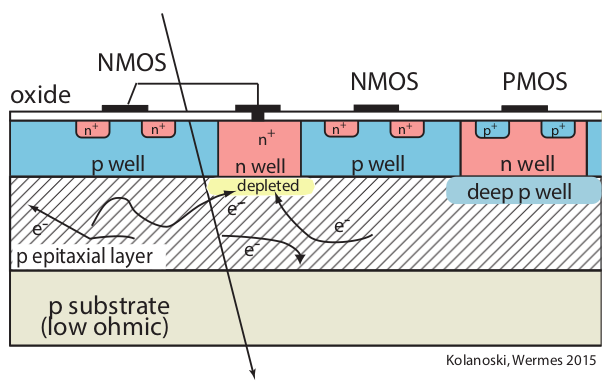
\includegraphics[width=.4\linewidth]{figures/MAPS_scheme.png}
   \caption{Concept cross section of MAPS and DMAPS pixel}
   \label{fig:MAPS_scheme}
\end{figure}
MAPS (figure a \ref{fig:MAPS_DMAPS_scheme}) have typically an epilayer in range 
1-20 $\mu m$ and because they
are not depleted, the charge is mainly collected by diffusion rather then by drift.
This makes the path of charges created in the bulk longer than usual and then they are
slow (of order of 100 ns) and the collection could be partial expecially after
an irradiation of the detector, when the trapping probability become highter. \\
DMAPS (figure b \ref{fig:MAPS_scheme}) are istead MAPS depleated 
with $d$ typically in $\sim$ 25-150 $\mu m$ (formula \ref{eq:deplation_d}),
si estende dal diodo al deep p well e certe volte, se ci sono stati backside process 
anche fino a dietro.\\
Both the sensors in the scheme  (figure \ref{fig:MAPS_scheme}) implement an n well as 
collection diode; to avoid the other n wells (which contain PMOS transistor) of the electronic circuit would compete 
in charge collection and to shield the CMOS circuit from the substrate, additionaly 
underlying deep p well are needed.\\
To implement a uniform and stronger electric field, DMAPS often uses large electrode
design (figure b \ref{fig:MAPS_scheme}) that requires multiple wells 
(typically four including deep n,p wells) and a new capacity term, that contributes to the 
total amplifier input capacity, adds on to the standard terms.
In addition to the capacity between pixels ($C_{pp}$) and
between the pixel and the backside ($C_{b}$), a non negligible contribution comes
from the capacities between wells ($C_{SW}$ and $C_{WW}$) needed to shield the
embedded electronics. These capacities affect the thermal and 1/f noise of the charge amplifier and
the $ \tau_{CSA}$ too:
\begin{multicols}{2}
   \begin{equation}
      ENC^2 _ {thermal} \propto \frac{4}{3}\frac{kT}{g_m}\frac{C_D ^2}{\tau_{sh}}
   \end{equation}\break
   \begin{equation}
     \tau_{CSA} \propto \frac{1}{g_m}\frac{C_D}{C_f}
   \end{equation}
\end{multicols}
where $g_m$ is the transconductance, $\tau_{sh}$ is the shaping time. \\
Coping with highter input capacity is simpler: il problema si pone davvero quando 
le intra well c sono grandi, allora potrebbe essere che il l'elettronica CMOS è 
accoppiata a queste capacità, e allora avresti cross talk.\\
\begin{figure}[h!]
   \centering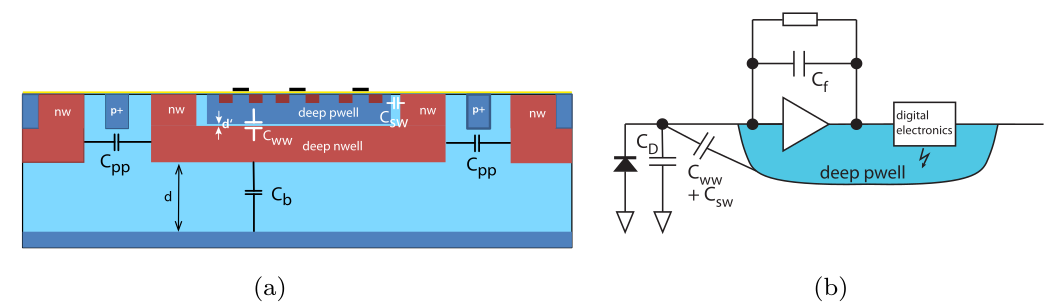
\includegraphics[width=12cm]{figures/DMAPS_capacity.png}
   \caption{$C_{pp}$, $C_{b}$, $C_{WW}$, $C_{SW}$}
   \label{fig:DMAPS_capacity}
\end{figure}

\subsubsection{DMAPS: large and small fill factor}
There are two different sensor-design approaches (figure \ref{fig:large_small_sensor_scheme})
to DMAPS:
\begin{itemize}
   \item large fill factor: a large collection electrode that is a large deep n-well
 and that host the embedded electronics
   \item small fill factor: a small n-well is used as charge collection node
\end{itemize}
Larger charge collection electrode sensors provide a uniform electric field in
the bulk that results in short drift path and so in good collection properties,
especially after irradiation, when trapping probability can become an issue. 
The drawback of a large fill-factor is the large
capacity ($\sim$100 fF): this contributes to the noise and to a
speed penalty and to a larger possibility of cross talk.
The small fill-factor variant, indeed, benefits from a small capacity (5-20 fF), but suffers 
from a not uniform electric field. \\
These two different types of sensor require different amplifier .
\begin{figure}
   \centering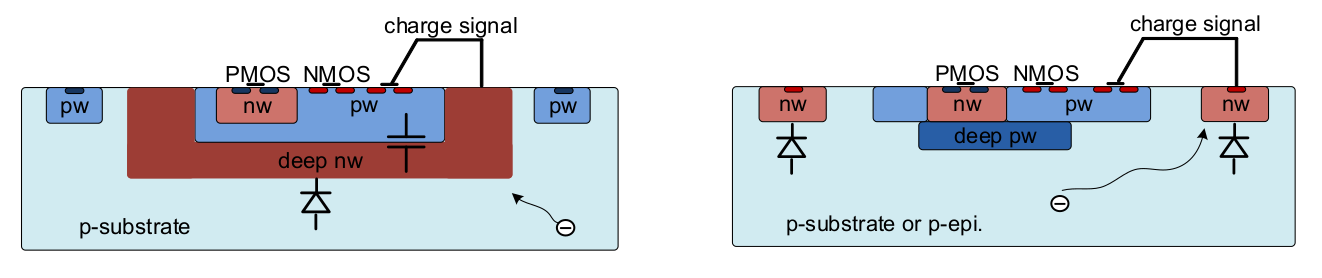
\includegraphics[width=12cm]{figures/large_small_sensor_scheme.png}
   \caption{Concept cross section with large and small fill factor}
   \label{fig:large_small_sensor_scheme}
\end{figure}

\begin{table}
   \begin{center}
   \begin{tabular}{|c | c |c |}
   \hline
   & small fill factor & large fill factor\\
   \hline
   \hline
   small sensor C & $\surd$ ($<$ 5 fF) & $\times$ ($\sim$ 100-200 fF)\\
   low noise & $\surd$ & $\times$\\
   low cross talk & $\surd$ & $\times$ \\
   velocity perfomances & $\surd$ & $\times$ ($\sim$ 100 ns)\\
   short drift paths & $\times$ & $\surd$ \\
   radiation hard & $\times$ & $\surd$ \\
   \hline
   \end{tabular}
   \caption{Small and large fill factor DMAPS characteristics}
   \label{tab:DMAPS_large_small_fillfactor}
   \end{center}
\end{table}

\subsubsection{A modified sensor}
A process modification that has become the standard solution that combine the carateristic
of a small fill factor sensor (small input amplifier capacity) and of large fill factor sensor
(uniform electric field) is the one carried out for ALICE upgrade (REFERENZA).\\
Una soluzione alternativa potrebbe essere fare pixel piccoli (E uniforme e c piccola), però 
così uno dovrebbe cambiare anche l'elettronica: non ci sarebbe posto per tutto. Il vantaggio
di questo modifica è proprio il fatto di non necessitare di nessun cambiamento nel layout,
tant'è vero che i chip di test spesso vengono fatti sia con che senza questa modifica.\\
The tecnique involve the implementation of a low dose implant in the epitassial layer in the 
upper part of the bulk.\\
Before the process modification the depletion region extends below the diode towards the 
substrate and it doesn't extend laterally so much even if a high bias is applied to 
the sensor (figure \ref{fig:modified_process}). \\
After, instead, two distinct pn junctions are built: one between the deep p well and the 
$n^-$ layer, and the other between the $n^-$ and the $p^-$ epitaxial layer, estendendosi a tutta l'area
planare del sensore.\\
Questa configurazione fa sì che si crei sotto l'elettrodo ($n^+$) si crei un minimo dove vengono 
accumulati anche dalle regione laterali gli elettroni. 
Il fatto che ci sia una zona di svuotamento dall'alto al basso che separi le zone drogate p, fa sì
che psub e pwell si possando polarizzare in modo diverso\footnote{This is true a meno di altre 
caratteristiche del sensore, come vedremo per MONOPIx1}.\\
La dose di drogaggio è importante: deve essere abbasatnza alta da prevalere sulla dose
dell'epitassial layer in modo da prevenire il punchthrought tra well e substrate e da 
prevenire l'inversione dopo alte fluenze (nell'articolo si mostra che il sensore modificato
tende ad avere migliori prestazioni anche dopo alte fluenze), ma anche abb bassa per poter essere svuotato 
a ragionevoli basse tensioni.\\
\begin{figure}
   \centering
   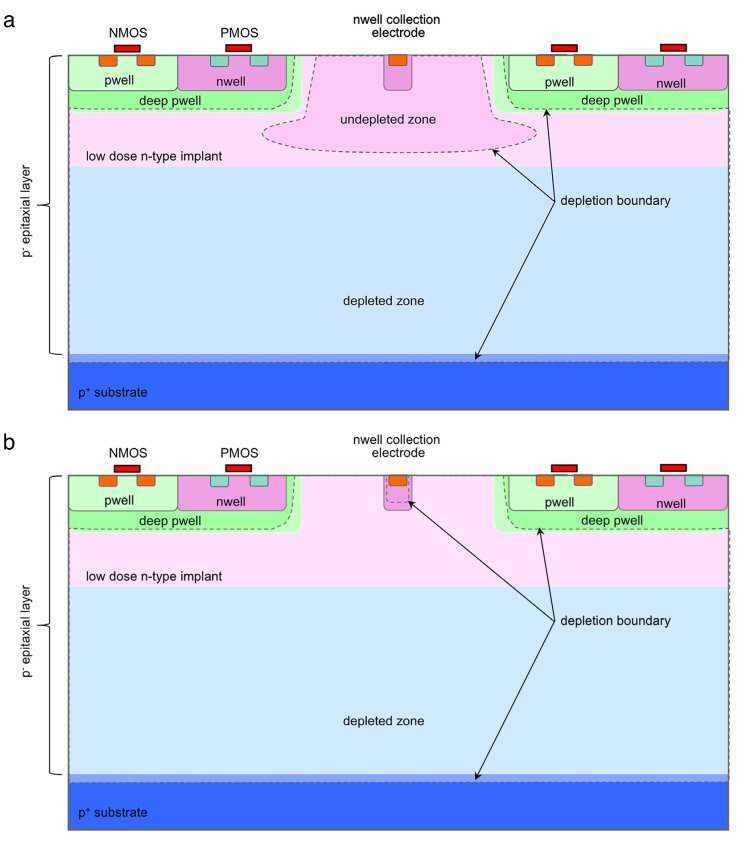
\includegraphics[width=.7\linewidth]{figures/modified_process.png}
   \caption{A modied process}
   \label{fig:modified_process}
\end{figure}


\subsection{Analog front end}
Dopo che la carica è stata creata nel substrato e abbia driftato fino agli elettrodi
inducendo un segnale su questi utlimi, il segnale creato entra nel circuito di FE 
(uno schema tipico di un circuito di FE in figura \ref{fig:readout_scheme}).
\begin{figure}
   \centering
   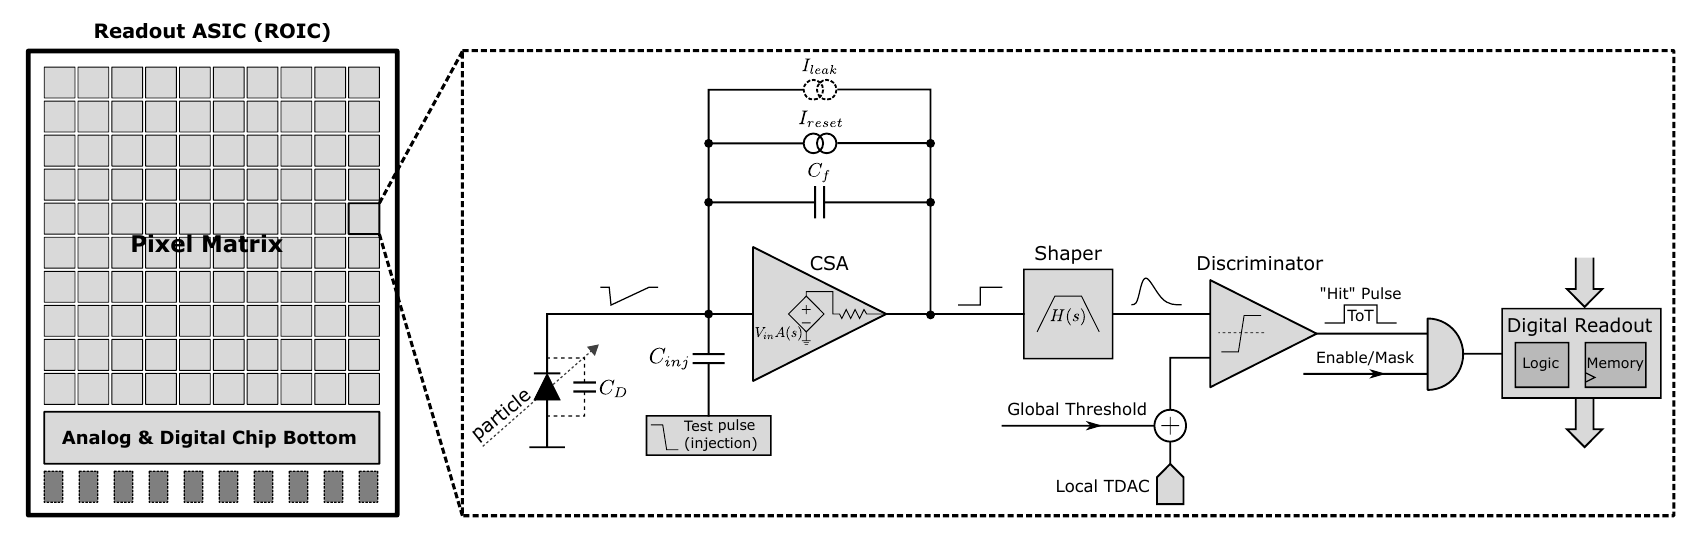
\includegraphics[width=1.\linewidth]{figures/readout_scheme.png}
   \caption{Readout FE scheme}
   \label{fig:readout_scheme}
\end{figure}
The main steps of the front end chain are: the preamplifier (that actually often is the 
only amplification stage) with a reset to the baseline mechanism, a shaper (a band-pass 
filter whose $\tau$ time costant is tuned in order to optimize S/N ratio and pile-up)
and finally a discriminator. The whole chain must be optimized to improve the S/N ratio.\\

\subsubsection{Preamplifier}
Even if circuits on the silicon crystal are only costruct by CMOSS, a
preamplifier can be modellized as an operational amplifier (OpAmp) with an impedence
feedback (first step in figure \ref{fig:readout_scheme}).\\
Depending on whether a capacity or a resistance is used as feedback, respectevely,
a charge or a voltage amplifier is used (figure ).
%\begin{figure}
   %centering
   %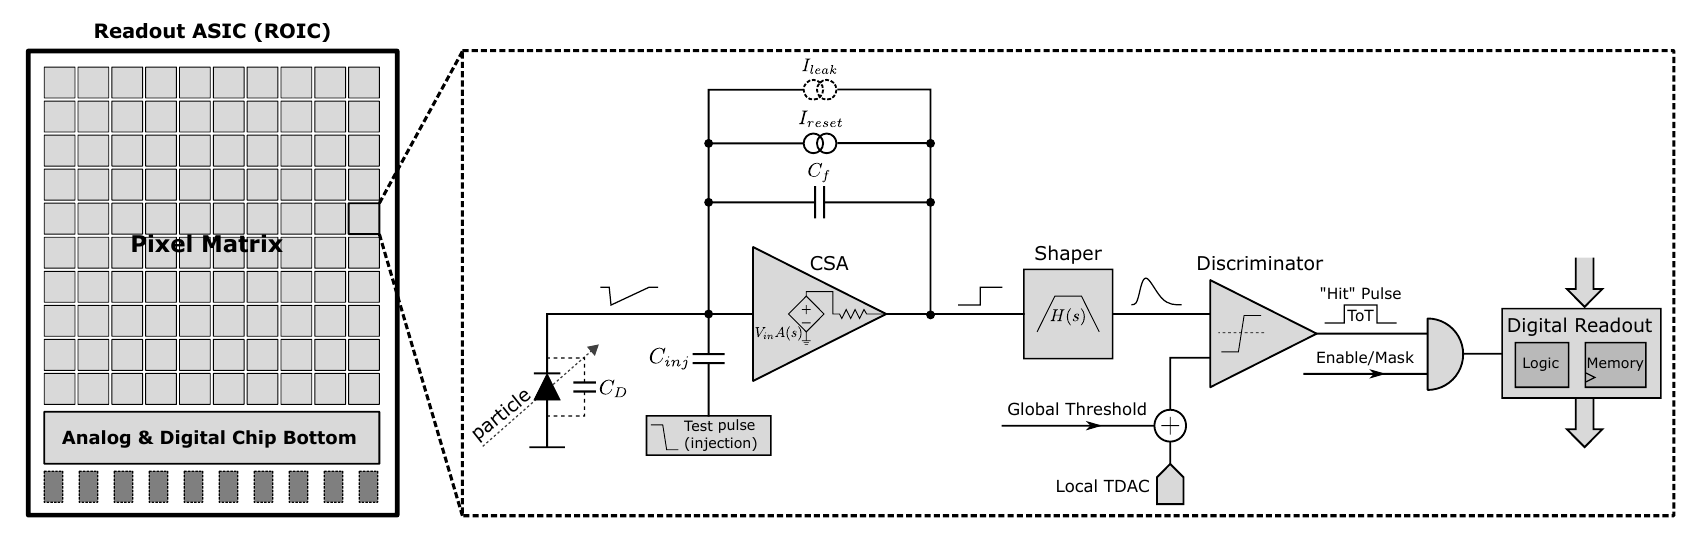
\includegraphics[width=1.\linewidth]{figures/readout_scheme.png}
   %\caption{Amplifier}
   %\label{fig:amplifier}
%\end{figure}
The amplification gain is determined by the input and feedback impedance:
\begin{equation}
   G = \frac{v_{out}}{v_{in}} = \frac{Z_{f}}{Z_{in}}
\end{equation}

If the signal duration is longer than the charateristic time ($R_S C_D$) of the amplifier with
a resistor in feedback ($\tau << \Delta t$), then the second condition in equation () is satisfied
and the system operates as a current amplifier:
\begin{equation}
   v_{out} = \frac{R_f}{R_S}v_{in}(t) = R_{f}i_{S}(t)
\end{equation}

When the S/N is small a charge amplifier is prefered.

\begin{equation}
   v_{out}(t) = -a_{0}v_{in}(t) =
\end{equation}

If the voltage input signals are large enought and have a sharp rise time, the voltage
sensistive preamplifier is often used. For this reason this preamplifier don't
perfectely suit to semiconductor detectors, especially for that one with large capacity
that also have large fill factor ($v_{in} = Q/C_{D} \approx$ 3fC/100 pF = 0.03 mV); on the other hand they are fine for that one with
very low capacity ($v_{in} = Q/C_{D} \approx$ 3fC/3 pF = 1 mV).

\subsubsection{ALPIDE-like front end}
ALPIDE (ALice PIxel DEtector) is the pixel detector (TowerJazz 180 nm CMOS) installed in the 
Inner Tracking System during the second long shut down of the LHC in 2019. Its FE became a
standard for all the following chip, and this also applies to ARCADIA MD1 and Monopix1, and this 
is why I'm going to explain some principals characteristics of how it works. 
\begin{figure}[h!]
   \centering
   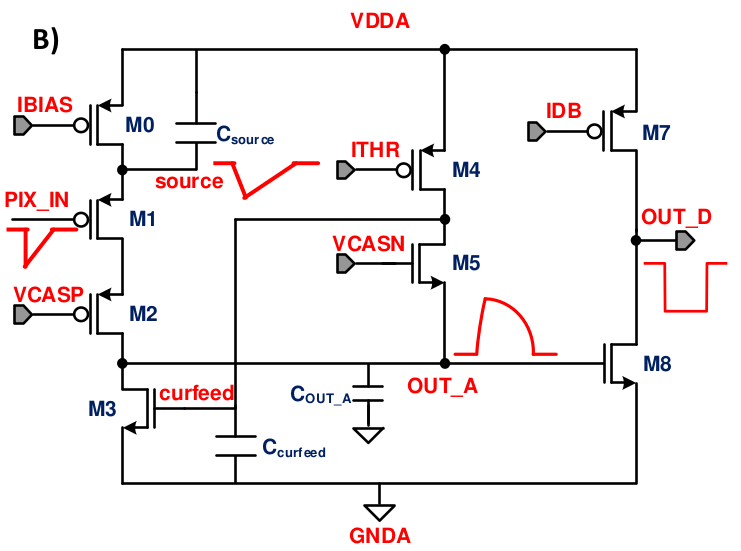
\includegraphics[width=.7\linewidth]{figures/ALPIDE_FE.png}
   \caption{ALPIDE like FE}
   \label{fig:ALPIDE-like}
\end{figure}
Carica fa un segnale negagtivo di $\Delta V_{PIX\_IN} = Q_{IN}/C_{IN}$ su PIX IN. 
M1 fa da source follower con IBIAS , costringendo la tensione al source a seguire la tensione di M1
al gate. \\
This causes transfer of charge 
$Q_{source}=C_{source}\Delta V_{PIXIN}$ from $C_{source}$ to $C_{OUT}$ in case the current sink
to GND is IBIAS.
So ideally:
\begin{equation}
   \Delta V_{OUT_A} = \frac{C_{Source}}{C_{OUTA}}\frac{Q_{IN}}{C_{IN}}
\end{equation}

A second branch (M4, M5) is used to generate a low frequency feedback. 
The voltage bias
VCASN and current bias ITHR define the baseline value of OUTA and the return to baseline after
a particle hit. The distance of the OUT A baseline voltage to the point where
IM8 = IDB defines the charge threshold.
  
\subsection{Readout logic}
One of the main problems of MAPS is the cross talk: one speaks about cross talk
when an input signal causes an output signal on neighbouring electrodes; digital signals
in the FE electronics do a lot of oscillations and digital switching produce spikes
and so noise.\\
METTI FORMULA DEL CROSS TALK E FAI VEDERE CHE PIÙ C È PICCOLA E MENO CROSS TALK HAI.\\
A way to partially resolve the problem, the analogical and digital part have different
bias channels and also the buses to MASS are different: this tecnique reduces the
loop in the circuit and therefore the induces singlas.\\


To store the analogical informations (charge collected, evolution of signal in time)
big buffers and a big bandwidth are needed.
Digital information, instead, means that if one pixel is hit 1 is recorded, and if
not 0 is recorded.\\
Typically one want to save some more information than the digital one, but also
less then the analogical one, so one choise used in some design is to save the time over threshold
(ToT) of the pulse; this is a a relatively coarse information (about 7 bits) but it
is correlated with the deposited charge by the impinging particle in the detector.

This is why, while the front end architecture remains similar from one generation
to the next (almost all pixels have a FE-ALPIDE), the processing of the information
produced by the front end, and the relationship of the front end to the rest of
the chip, changed significantly.\\
Il modo con cui vengono lette le hit su una matrice è il column drain readout.\\
The simple 3T (three transistor) readout has a row select, a
source-follower buffer and an input baseline reset;

Moreover the readout architetcture can be full, if every hit from every pixel must eventually
make its way to the data output, or triggered, if hits are recorded during a trigger signal.
Again, on the one hand the triggered-readout needs buffers and storage memories
(therfore needs space on the pixel are to accomodate them), on the other the full readout,
because there is no need to store hit data on chip, needs an high enough bandwidth.\\
I will now give some hints about the optimization between this two trends.

If all the pixels in a column share a data bus to the EoC and only one pixel at a time can
be use and there aren't any storage memory, the column (si comporta) as a single
server queue and the probability for waiting a time greater than $t$ with an input
hit rate $\mu$ in a column and an output bandwidt $B_W$ is:
\begin{equation}
P(T > t) = \frac{\mu}{B_W} e^{-( B_W-\mu )t}
\end{equation}
To avoid hit loss (let's neglect the contribution to the inefficency of the dead
time $\tau$), for example imponing $P(T > t)\sim$0.001, one obtains
$(B_W -\mu)t_t\sim$6, where $t_t$ is the time to transfer the hit;
since $t_t$ is small, one must have $B_W \gg \mu$, that means a high bandwidth.

If shift registers (SR) are used to transfer data instead of buses the bandwidth $B_W$
of the SR corresponds to the clock speed; differently from the bus case, each pixel
sees a different bandwidth depending on the position on the queue: the first pixel
in the priority logic chain , that is the closest pixel to the EoC typically,
sees a full bandwidth, but the next pixel sees less bandwidth because
occasionally it will be blocked by data from the previou pixel.\\
Then the condition about the bandwidth and the hit rate become: $B_{W,i} > \mu_{i}$,
where the index $i$ means the requirement is for a single pixel. If all the pixels
on the same column
have the same rate $\mu = N\mu_{i}$ and the condition become $B_{W} > \mu$.
The bandwidth must be chosen such that the mean time between hits of the last pixel
in the readout chain is bigger than that.\\
Questa condizione tra banda e rate sulla colonna ci dice già una cosa importante:
il fatto che l'algoritmo di lettura column drain non è scalabile: infatti se aumento
il numero di pixel sulla stessa linea di lettura rischio di violare la condizione.\\
La scalabilità risiede quindi nel poter utilizzare tanti chip piccoli.\\


If instead the hits are stored in buffers until a trigger signal arrives, the input rate
to column bus is reduced as $\mu'=\mu t$, where $t$ is the trigger rate.
This implies that $B_{W} \gtrsim \mu'$, that is a very relaxed condition on the
bandwidth, but the limiting factor is the amount of memory  which the pixel area
can host; the amount needed depends on the trigger frequency 1/$t$ as
$\propto\mu/t$, that means that the highter the trigger frequency and the highter
the hit rate that can be handled. \\
In order to have an efficient use of memory on pixel area it's convenient
grouping pixels into regions with shared storage. Let's look what happens when
single pixel local storage is used: for example, suppose to have a 50 kHz single
pixel hits rate and a trigger frequency of 1/5 microseconds, allora il rapporto dei due
è 0.25 e cioè il numero medio di hit perse per trigger signal.\\
usando la statistica di Poisson, uno dovrebbe storare 3 hit per pixel se volesse
raggiungere il 99.9 per cento di efficienza.\\
Consideriamo cosa succede se faccio un gruppo di quattro pixel: allora se il rate
medio di 1 hit sui 4 pixel (sempre 50 khz di single pixel) per ogni trigger signal, allora se volessi un'eff di 99.9
avrei bisogno di un buffer depht of 5 region-hits. Quindi significa che in media per
ogni pixel avrei 5/4 = 1.25 buffer depht, minore di quello di prima.\\
L'architettura di lettura che colloca i pixel in regioni da 4 si chiama FE-I4.\\

One standard way to reduce the readout bandwidth is to implement the zero suppression
on the pixel: only informations about channels with an hit (when signal exceeds
the discriminator threshold) are read.

Per gli esperimenti agli acceleratori, e soprattutto per gli esperimenti che
intendono aumentare la luminosita, è sicuramente di particolare importanza
l'occupancy dei pixel: sia il rate del noise va mantenuto basso, sia un
bisogna prestare attenzione al pile up.
L'occupancy tra le altre cose dipende dalla differenza tra threshold e offset del
segnale, per cui uno può agire sulla soglia per poterla cambiare.\\
FORMULA? slide APSEL\\
Una soluzione potrebbe essere mettere un trigger e in sincro con il beam mettere
il reset avviene ad ogni beam collision; questo consuma però un sacco di power. \\

\begin{comment}

\end{comment}
\end{titlepage}
